% Бүлэг 2

\chapter{Багшийн журнал вэб системийн хөгжүүлэлт} % Бүлгийн нэр
\label{Chapter2} % Энэ бүлэг рүү ишлэл хийх бол \ref{Chapter1} командыг ашигла 

\section{Системийн үйл ажиллагааны тухай дэлгэрэнгүй }
Энэхүү систем нь ЕБС-ийн бүх сургуулиудад хэрэглэж болох бөгөөд улсын төсвөөс гарч буй журнал хэвлэлтийн зардал, багшийн ажлын цаг, тухайн сургуулийн үйл ажиллагааг хялбарчлах, өөрийн онцлогт тохируулан хэрэглэх боломжтой байна. Энэхүү цахим журналыг хэрэглэснээр сургуулийн удирдлага, багш, сурагч, эцэг эхийн хооронд мэдээлэл солилцоход хялбар болох бөгөөд цаг тухай бүрд нь мэдээллээр хангах боломжтой болох юм.

\section{Системийг ашиглах хэрэглэгчид}
Ерөнхий боловсролын сургалттай бүх сургуулиуд хэрэглэх боломжтой.
Жишээ нь: 
\begin{itemize}
\item Улсын хэмжээний бүх сургууль
\item Ерөнхий боловсрол олгодог хувийн сургуулиуд
\end{itemize}
\section{Функционал шаардлага}
 Энэхүү веб нь админ/сургалтын менежер/, багш, сурагч, эцэг эх гэсэн 4-н оролцогчтой.
Админ/сургалтын менежер/ нь: Бүх хуудсыг хянах, бүртгэлтэй багш, сурагчдын ерөнхий мэдээллийг удирдах.
Багш: Суралцагчийн дэлгэрэнгүй мэдээлэл оруулах, хичээлтэй холбоотой мэдээлэл оруулах түүнийгээ эцэг эхчүүдтэй явуулах.
Сурагч: Мэдээллийг харах,сэтгэгдэл бичих боломжтой.
Эцэг эх: Мэдээллийг харах,сэтгэгдэл бичих, шаардлагатай үед санал хүсэлт бичих боломжтой.\\
Админ/сургалтын менежер/ функциональ шаардлага:
\begin{enumerate}
	\item Багшийн бүртгэлийн мэдээлэл
	%\begin{enumerate}
	%	\item[1.1] Багш нэмэх
	%	\item[1.2] Багш хасах
	%	\item[1.3] Засварлах
	%\end{enumerate}
	\item Суралцагчийн бүртэглийн мэдээлэл
	%\begin{enumerate}
	%	\item[2.1] Сурагч нэмэх
	%	\item[2.2] Суралцагчийн шилжилт хөдөлгөөн
	%	\item[2.3] Засварлах
	%\end{enumerate}
	\item Хичээлийн бүртгэлийн мэдээлэл
	\item Ангийн мэдээлэл
	\item Тайлан
	\begin{enumerate}
		\item[6.1] Ангийн тайлан
		\item[6.2] Суралцагчийн тайлан
		\item[6.3] Багшийн хичээлийн тайлан
		\item[6.4] Ирцийн тайлан
	\end{enumerate}
	\item Сургуулийн мэдээлэл
	%\item Зочдын сэтгэгдэлд хариу бичих
\end{enumerate}
Багшийн функциональ шаардлага:
\begin{enumerate}
	\item Суралцагчийн мэдээлэл оруулах
	\begin{enumerate}
		\item[1.1] Дэлгэрэнгүй мэдээлэл оруулах
		\item[1.2] Хичээлээс гадуурх суралцагчтай холбоотой мэдээлэл оруулах
	\end{enumerate}
	\item Суралцагчийн ирц, үнэлгээ
	\item Эцэг эхийн бүртгэл хийх
	%\begin{enumerate}
	%	\item[3.1] Нэмэх
	%	\item[3.2] Хасах
	%	\item[3.3] Засах
	%\end{enumerate}
	\item Хичээлийн мэдээлэл
	%\begin{enumerate}
	%	\item[4.1] Сэдэв нэмэх
	%	\item[4.2] Сэдэв хасах
	%	\item[4.3] Засварлах
	%\end{enumerate}
	\item Багшийн тэмдэглэл оруулах
	%\begin{enumerate}
	%	\item[5.1] Тэмдэглэл нэмэх
	%	\item[5.2] Тэмдэглэл хасах
	%	\item[5.3] Засварлах
	%\end{enumerate}
\end{enumerate}
Суралцагчийн функциональ шаардлага
\begin{enumerate}
	\item Мэдээллээ харах
	\begin{enumerate}
		\item[1.1] Үндсэн мэдээлэл
		\item[1.2] Ирц, үнэлгээ
		\item[1.3] Хичээлээс гадуурх суралцагчтай холбоотой мэдээлэл
	\end{enumerate}
	\item Тэмдэглэл
	%\begin{enumerate}
	%	\item[2.1] Ирсэн тэмдэглэл
	%	\item[2.2] Тэмдэглэл бичих
	%\end{enumerate}
\end{enumerate}
Эцэг эхийн функциональ шаардлага
\begin{enumerate}
	\item Мэдээллээ харах
	\begin{enumerate}
		\item[1.1] Үндсэн мэдээлэл
		\item[1.2] Хүүхдийнхээ ирц, үнэлгээ
		\item[1.3] Хичээлээс гадуурх суралцагчтай холбоотой мэдээлэл
	\end{enumerate}
	\item Тэмдэглэл
	%\begin{enumerate}
	%	\item[2.1] Ирсэн тэмдэглэл
	%	\item[2.2] Тэмдэглэл бичих
	%\end{enumerate}
\end{enumerate}
\section{Функционал бус шаардлага}
\begin{enumerate}
	\item Өгөгдлийн сан ачааллах хугацаа нь хурдан шуурхай байх. Бүх өгөгдлүүд өгөгдлийн санд хадгалагдсан байх болно
	\item Вебд 1000-с 10000-хүн нэгэн зэрэг хандаж үйл ажиллагаа явуулах учир серверийн хүчин өндөр байх
	\item Архитектурын хувьд windows орчинд хөгжүүлэгдэнэ.Вебийн хөгжүүлэлт нь CodeIgniter framework – той хамтран ажиллаж боломжтой хэлүүд дээр хийгдэнэ.
	\item Кодчилолын хувьд CodeIgniter framework –ийн стандартын дагуу хийгдэнэ.
\end{enumerate}
\section{Юзкейс диаграм}
\begin{figure}[htbp]
	\centering
	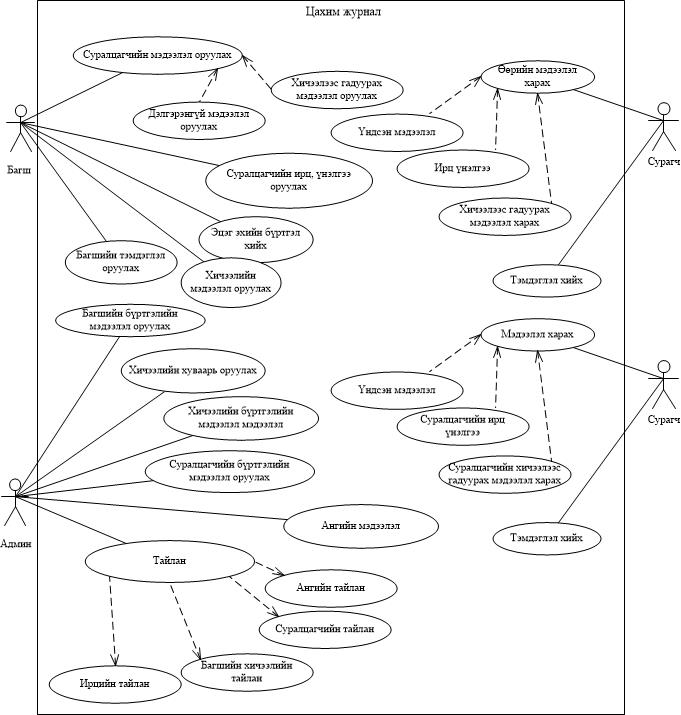
\includegraphics[scale=0.8]{Diagrams/UseCase}
	\caption[Юзкейс диаграм]{Юзкейс диаграм}
	\label{fit:UseCase}
\end{figure}
%-------------------------------------------------------------------------------------------------------
\section{Юзкейс диаграмын тодорхойлолт}
\begin{center}
	\begin{table}[!htbp]
		\caption{}
		\begin{tabular}{|p{4cm}|p{11cm}|}
		\hline
			Нэр: & Суралцагчийн бүртгэлийн мэдээлэл \\
		\hline
			ID: & 1 \\
		\hline
			Товч тайлбар: & Суралцагчийг веб серверд шинээр бүртгэл үүсгэнэ. \\
		\hline
			Триггер: & Суралцагчийн бүртгүүлэх шаардлагатай болсон. \\
		\hline
			Үндсэн оролцогч: & Суралцагч \\
		\hline
			Хоёрдогч оролцогч: & Эцэг эх  \\
		\hline
			Өмнөх нөхцөл: &  Веб сервер ажиллагаатай байх\\
		\hline
			Ажлын урсгал: & \begin{enumerate}
						 	\item Суралцагч нь бүртгүүлэхийг сонгосноор энэ юз кейс эхлэнэ. 
						 	\item Веб сервер нь суралцагчид бүртгүүлэх цонхыг харуулна.  
						 	\item Веб сервер нь админ оруулсан мэдээллийг шалгана. 
						 	\item IF (“мэдээлэл үнэн зөв бол”)
							 	\begin{enumerate}
							 		\item[5.1] Веб сервер админы оруулсан мэдээллийг баазад хадгална.
							 		\item[5.2] Веб сервер Суралцагчийг амжилттай бүртгүүлсэнийг нь харуулна. 
							 	\end{enumerate}
						 	\item ELSE
							 	\begin{enumerate}
							 		\item[6.1] Веб сервер нь админы оруулсан мэдээлэл бүрийг шалгана.  
							 		\item[6.2] Веб сервер нь алдаатай оруулсан мэдээллийг тодруулж харуулна. 
							 		\item[6.3] Веб сервер нь мэдээллийг дахин оруулахыг асууна. 
							 	\end{enumerate}
						  \end{enumerate}
\\					  \hline
				Дараах нөхцөл: &
				 \begin{enumerate}
									\item Суралцагч веб серверд бүртгэлтэй болсон байна. 
									\item Суралцагчийн мэдээлэл баазад хадгалагдсан байна. 
				\end{enumerate}	   
\\				   \hline
				Альтернатив урсгал: &  \begin{enumerate}
									\item Веб сервер дээр алдаа гарсан. 
										\end{enumerate}
				\\	\hline
		\end{tabular}
	\end{table}
\end{center}


\begin{center}
	\begin{table}[!htbp]
		\caption{}
		\begin{tabular}{|p{4cm}|p{11cm}|}
			\hline
			Нэр: & Багшийн бүртгэлийн мэдээлэл оруулах \\
			\hline
			ID: & 2 \\
			\hline
			Товч тайлбар: & Админ веб серверд шинээр багш нэмэж оруудах\\
			\hline
			Триггер: & Багшийг бүртгэх шаардлагатай болсон. \\
			\hline
			Үндсэн оролцогч: & Админ \\
			\hline
			Хоёрдогч оролцогч: & Багш  \\
			\hline
				Өмнөх нөхцөл: &  Веб сервер ажиллагаатай байх\\
			\hline
			Ажлын урсгал: & \begin{enumerate}
				\item Багш нь бүртгүүлэхийг сонгосноор энэ юз кейс эхлэнэ. 
				\item Веб сервер нь админд бүртгүүлэх цонхыг харуулна.  
				\item Веб сервер нь админы оруулсан мэдээллийг шалгана. 
				\item IF (“мэдээлэл үнэн зөв бол”)
				\begin{enumerate}
					\item[5.1] Веб сервер админы оруулсан мэдээллийг баазад хадгална.
					\item[5.2] Веб сервер Багшийг амжилттай бүртгүүлсэнийг нь харуулна. 
				\end{enumerate}
				\item ELSE
				\begin{enumerate}
					\item[6.1] Веб сервер нь админы оруулсан мэдээлэл бүрийг шалгана.  
					\item[6.2] Веб сервер нь алдаатай оруулсан мэдээллийг тодруулж харуулна. 
					\item[6.3] Веб сервер нь мэдээллийг дахин оруулахыг асууна. 
				\end{enumerate}
			\end{enumerate}
			\\					  \hline
			Дараах нөхцөл: &
			\begin{enumerate}
				\item Багш веб серверд бүртгэлтэй болсон байна. 
				\item Багшийн мэдээлэл баазад хадгалагдсан байна. 
			\end{enumerate}	   
			\\				   \hline
			Альтернатив урсгал: &  \begin{enumerate}
				\item Веб сервер дээр алдаа гарсан. 
			\end{enumerate}
			\\	\hline
		\end{tabular}
	\end{table}
\end{center}

\begin{center}
	\begin{table}[!htbp]
		\caption{}
		\begin{tabular}{|p{4cm}|p{11cm}|}
			\hline
			Нэр: & Арга хэмжээ зарлах \\
			\hline
			ID: & 3 \\
			\hline
			Товч тайлбар: & Хэрэглэгч өөрийн хуудсаар дамжуулан удахгүй болох арга хэмжээг зарлана.  \\
			\hline
			Триггер: & Хэрэглэгч арга хэмжээ зарлахыг хүссэн. \\
			\hline
			Үндсэн оролцогч: & Хэрэглэгч \\
			\hline
			Хоёрдогч оролцогч: & Байхгүй  \\
			\hline
			Өмнөх нөхцөл: &  \begin{enumerate}
				\item Вебд  өөрийн хуудсаа нээсэн байх.
				\item Веб хэвийн ажиллагаатай байх.
			\end{enumerate}
			\\			\hline
			Ажлын урсгал: & \begin{enumerate}
								\item Хэрэглэгч арга хэмжээ зарлах хэсгийг сонгосоноор энэхүү энэ юзкейс эхэлнэ.
								\item Веб арга хэмжээний тухай бөглөх хуудсыг харуулна
								\item Хэрэглэгч хуудсийг (арга хэмжээ эхлэх, дуусах огноо, тайлбар ) бөглөнө.
								\item IF( Мэдээлэл үнэн бөглөсөн бол )
									\begin{enumerate}
										\item[4.1] Веб арга хэмжээ баталгаажуулах хэсгийг харуулна
									\end{enumerate}
								\item ELSE 
									\begin{enumerate}
										\item[5.1] Веб хэрэглэгчийн оруулсан мэдээлэл алдаатайг мэдэгдэнэ.
										\item[5.2] Хэрэглэгч хуудсыг дахин бөглөнө.
									\end{enumerate}
								\item Хэрэглэгч арга хэмжээг баталгаажуулах хэсгийг сонгоно.
								\item Веб арга хэмжээ амжилттай баталгаажсаныг мэдэгдэнэ.
							\end{enumerate}
\\						\hline
			Дараах нөхцөл: & Арга хэмжээ зарлагдсан байна. \\
			\hline
			Альтернатив урсгал: & Хэрэглэгч арга хэмжээг цуцалсан байна. \\
			\hline
		\end{tabular}
	\end{table}
\end{center}


\begin{center}
	\begin{table}[!htbp]
		\caption{}
		\begin{tabular}{|p{4cm}|p{11cm}|}
			\hline
			Нэр: & Зочинтой харилцах \\
			\hline
			ID: & 4 \\
			\hline
			Товч тайлбар: & Хуудасанд үлдээсэн зочины сэтгэгдэлд хариу бичих.  \\
			\hline
			Үндсэн оролцогч: & Хэрэглэгч \\
			\hline
			Хоёрдогч оролцогч: & Зочин  \\
			\hline
			Өмнөх нөхцөл: &  \begin{enumerate}
				\item Өөрийн хуудсанд нэвтэрсэн байх.
				\item Сэтгэгдэл үлдээсэн зочин вебд бүртгэлтэй байх.
			\end{enumerate}
			\\			\hline
			Ажлын урсгал: & \begin{enumerate}
								\item Хэрэглэгч зочины үлдээсэн сэтгэгдэлд хариу бичих хэсгийг сонгосоноор энэ юзкейс эхэлнэ.
								\item Веб хариу бичих талбарыг нээж харуулна.
								\item Хэрэглэгч зочины сэтгэгдэлд хариу бичнэ.
								\item Хэрэглэгч хариу сэтгэгдэлээ илгээнэ.
								\item Веб хариу сэтгэгдэл амжилттай илгээгдсэнийг мэдэгдэнэ.
							\end{enumerate} \\
						\hline
			Дараах нөхцөл: & Хэрэглэгч зочины сэтгэгдэлд хариу бичсэн байна. \\
			\hline
			Альтернатив урсгал: & Хэрэглэгч бичсэн сэтгэгдэлээ устгасан байна. \\
			\hline
		\end{tabular}
	\end{table}
\end{center}

\begin{center}
	\begin{table}[!htbp]
		\caption{}
		\begin{tabular}{|p{4cm}|p{11cm}|}
			\hline
			Нэр: & Реклам зар сурталчилгаа харах  \\
			\hline
			ID: & 5 \\
			\hline
			Товч тайлбар: & Зочин вебийн реклам зар сурталчилгааг харна.  \\
			\hline
			Үндсэн оролцогч: & Зочин \\
			\hline
			Хоёрдогч оролцогч: & Байхгүй  \\
			\hline
			Өмнөх нөхцөл: &  Вебд нэвтэрсэн байх \\
			\hline
			Ажлын урсгал: &  \begin{enumerate}
								\item Зочин вебд реклам зар сурталчилгаа харах зорилготой нэвтэрсэнээр энэ юзкейс эхэлнэ.
								\item Веб реклам зар сурталчилгааны төрлүүдийг харуулна. 
								\item Зочин реклам зар сурталчилгааныхаа төрлөө сонгоно сонгоно.
								\item Веб зочины сонгосон төрлийг харуулна.  
							\end{enumerate}	 \\
						\hline
			Дараах нөхцөл: & Зочин реклам зар сурталчилгаа харсан байна \\
			\hline 
			Альтернатив урсгал: & Байхгүй \\
			\hline
		\end{tabular}
	\end{table}
\end{center}

\begin{center}
	\begin{table}[!htbp]
		\caption{} 
		\begin{tabular}{|p{4cm}|p{11cm}|}
			\hline
			Нэр: & Сэтгэгдэл бичих  \\
			\hline
			ID: & 6 \\
			\hline
			Товч тайлбар: & Зочин хуудсанд сэтгэгдэл үлдээх.  \\
			\hline
			Үндсэн оролцогч: & Зочин \\
			\hline
			Хоёрдогч оролцогч: & Байхгүй  \\
			\hline
			Өмнөх нөхцөл: &  Вебд бүртгэлтэй байх \\
			\hline
			Ажлын урсгал: & \begin{enumerate}
								\item Зочин сэтгэгдэл үлдээх хэсгийг сонгосоноор энэ юзкейс эхэлнэ
								\item Веб зочинд сэтгэгдэл үлдээх хэсгийг харуулна
								\item Зочин хэсгийг сонгоно
								\item IF( Зочин вебд бүртгэлгүй бол )
									\begin{enumerate}
										\item[4.1] Веб бүртгэлийн хуудсийг харуулна
									\end{enumerate}
								\item ELSE
									\begin{enumerate}
										\item[5.1] Зочин сэтгэгдэл үлдээх хэсэгт сэтгэгдэлээ үлдээнэ
									\end{enumerate}
								\item Зочин сэтгэгдэл баталгаажуулах хэсгийг сонгоно
								\item Веб сэтгэгдэл амжилттай үлдээснийг мэдэгдэнэ.
							\end{enumerate} 	
\\				\hline
			Дараах нөхцөл: & Зочин хуудсанд сэтгэгдэл үлдээсэн байна. \\
			\hline
			Альтернатив урсгал: & Зочин сэтгэгдэлээ устгасан байна. \\
			\hline
		\end{tabular}
	\end{table}
\end{center}

\begin{center}
	\begin{table}[!htbp]
		\caption{} 
		\begin{tabular}{|p{4cm}|p{11cm}|}
			\hline
			Нэр: & Хайлт хийх  \\
			\hline
			ID: & 7 \\
			\hline
			Товч тайлбар: & Зочин вебээс өөрийн хүссэн реклам зар сурталчилгааг хайна.  \\
			\hline
			Үндсэн оролцогч: & Зочин \\
			\hline
			Хоёрдогч оролцогч: & Байхгүй  \\
			\hline
			Өмнөх нөхцөл: &  Вебд нэвтэрсэн байх \\
			\hline
			Ажлын урсгал: & \begin{enumerate}
								\item Зочин хайлт хийх хэсгийг сонгосоноор энэхүү юзкейс эхэлнэ
								\item Веб хайлт хийх төрлүүдийг харуулна харуулна
								\item Зочин хайлт хийх төрөлөө сонгоно
								\item Веб зочины сонгосон хайлт хийх хэсгийг харуулна
								\item Зочин хайлтын утгаа оруулна
								\item IF(Хайлтын утга алдаатай бол)
									\begin{enumerate}
										\item[6.1] Веб хайлтын утга алдаатайг зочинд мэдэгдэнэ.
										\item[6.2] Веб зочинд зөв хайлтын жишээ утга харуулна
									\end{enumerate}	
								\item ELSE IF(Таны хайсан утга )
									\begin{enumerate}
										\item[7.1] Веб таны хайсан утга илэрцгүй 
									\end{enumerate}
								\item Зочин хайлтанд илэрсэн утгуудыг харуулна
							\end{enumerate} 	\\
						\hline
			Дараах нөхцөл: & Зочин вебээс хүссэн хайлтаа олсон байна. \\
			\hline
			Альтернатив урсгал: & Зочины хайлт илэрцгүй байна.\\
			\hline
		\end{tabular}
	\end{table}
\end{center}

\begin{center}
\begin{table}[!htbp]
	\caption{}
	\begin{tabular}{|p{4cm}|p{11cm}|}
		\hline
		Нэр: & Арга хэмжээнд санал өгөх  \\
		\hline
		ID: & 8 \\
		\hline
		Товч тайлбар: & Зочин хуудсануудын арга хэмжээнд санал өгөх боломжтой.  \\
		\hline
		Үндсэн оролцогч: & Зочин \\
		\hline
		Хоёрдогч оролцогч: & Байхгүй  \\
		\hline
		Өмнөх нөхцөл: &  Зочин вебд бүртгэлтэй байх. \\
		\hline
		Ажлын урсгал: & \begin{enumerate}
							\item Зочин арга хэмжээнд санал өгөх хэсгийг сонгосоноор энэ юзкейс эхэлнэ.
							\item Веб арга хэмжээнд санал өгөх хэсгийг харуулна
							\item Зочин санал өгөх хэсгийг сонгоно.
							\item IF( Зочин вебд бүртгэлгүй бол )
								\begin{enumerate}
									\item[4.1] Веб бүртгэлийн хуудсийг харуулна
								\end{enumerate}
							\item ELSE
								\begin{enumerate}
									\item[5.1] Зочин арга хэмжээнд санал өгнө
								\end{enumerate}
							\item Зочин санал баталгаажсаны веб мэдэгдэнэ
						\end{enumerate}	\\
		\hline
		Дараах нөхцөл: & Зочин арга хэмжээнд санал өгсөн байна. \\
		\hline
		Альтернатив урсгал: & Зочин саналаа устгасан байна. \\
		\hline
	\end{tabular}
\end{table}
\end{center}

\begin{center}
	\begin{table}[!htbp]
		\caption{}
		\begin{tabular}{|p{4cm}|p{11cm}|}
			\hline
			Нэр: & Бүртгэлтэй хэрэглэгч удирдах  \\
			\hline
			ID: & 9 \\
			\hline
			Товч тайлбар: & Админ бүртгэлтэй зочиныг вебээс хасах.  \\
			\hline
			Үндсэн оролцогч: & Админ \\
			\hline
			Хоёрдогч оролцогч: & Байхгүй  \\
			\hline
			Өмнөх нөхцөл: &  Зочин вебд зүй зохисгүй зүйл хийх. \\
			\hline
			Ажлын урсгал: & \begin{enumerate}
								\item Админ бүртгэлтэй зочидын жагсаалтыг сонгосоноор энэ юзкейс эхэлнэ.
								\item Веб бүртгэлтэй зочидын жагсаалтыг харуулна
								\item Админ зөрчилтэй зочинг сонгоно
								\item Веб зөрчилтэй зочины мэдээллийг харуулна
								\item Админ зөрчилтэй зочинг вебээс хасна
								\item Веб зөрчилтэй зочин амжилттэй вебээс хасагдсаныг мэдэгдэнэ.
							\end{enumerate}	\\
						\hline
			Дараах нөхцөл: & Зөрчилтэй зочин вебээс хасагдсан байна.(Бүртгэлтэй зочидын сангаас хасагдах ) \\
			\hline
			Альтернатив урсгал: & Админ зочинг буцаан сэргээсэн байна. \\
			\hline
		\end{tabular}
	\end{table}
\end{center}

\begin{center}
	\begin{table}[!htbp]
		\caption{}
		\begin{tabular}{|p{4cm}|p{11cm}|}
			\hline
			Нэр: & Сайтын ерөнхий реклам зар сурталчилгааг удирдах  \\
			\hline
			ID: & 10 \\
			\hline
			Товч тайлбар: & Сайтын ерөнхий реклам зар сурталчилгааг нэмэх, хасах, өөрчлөх боломжтой.  \\
			\hline
			Үндсэн оролцогч: & Админ \\
			\hline
			Хоёрдогч оролцогч: & Байхгүй  \\
			\hline
			Өмнөх нөхцөл: &  Админ эрхээр нэвтэрсэн байх. \\
			\hline
			Ажлын урсгал: & \begin{enumerate}
								\item Админ сайтын ерөнхий реклам зар сурталчилгаа удирдах хэсгийг сонгосоноор энэ юзкейс эхэлнэ
								\item Веб реклам зар сурталчилгаа удирдах төрлүүдийг харуулна
								\item Админ реклам зар сурталчилгаа нэмэх хэсгийг сонгоно
								\item Веб нь реклам зар сурталчилгаа нэмэх хуудсыг админд харуулна.
								\item Админ реклам зар сурталчилгааныхаа замыг зааж өгнө.
								\item Веб тухайн реклам зар сурталчилгаа мөн эсэхийг шалгана.
								\item IF (реклам зар сурталчилгаа байгаа бол)
									\begin{enumerate}
										\item[7.1] Веб тухайн реклам зар сурталчилгааг баазруу ачаална.
										\item[7.2] IF (амжилттай ачаалагдсан бол)
											\begin{enumerate}
												\item[7.2.1] Амжилттай ачаалагдсан мэдээллийг админд харуулна. 
											\end{enumerate}
										\item[7.3] Else
											\begin{enumerate}
												\item[7.3.1] Веб ачаалах үеийн алдааг админд харуулна. 
											\end{enumerate}
										\item[7.4] Веб зөв зам дахин оруулахыг асууна.
									\end{enumerate}
								\item Вебийн ерөнхий реклам зар сурталчилгаа амжилттай нэмэгдсэнийг мэдэгдэнэ.
						\end{enumerate}	\\
					\hline
			Дараах нөхцөл: & Вебийн ерөнхий реклам зар сурталчилгаа нэмэгдсэн байна \\
			\hline
			Альтернатив урсгал: & Админ буцааж устгасан байна \\
			\hline
		\end{tabular}
	\end{table}
\end{center}

%-------------------------------------------------------------------------------
\section{Шинжилгээний класс диаграм}

\begin{figure}[ht]
	\centering
	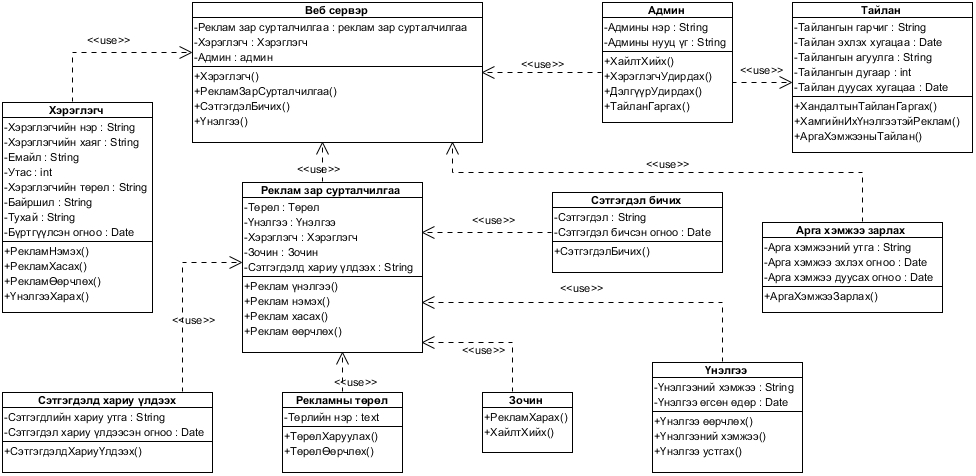
\includegraphics[angle=90,scale=0.7]{Diagrams/SClass}
	\caption[Шинжилгээний класс диаграм]{Шинжилгээний класс диаграм}
	\label{fig:SClass}
\end{figure}

%--------------------------------------------------------------
\section{Шинжилгээний дарааллын диаграм}
\begin{figure}
	\centering
	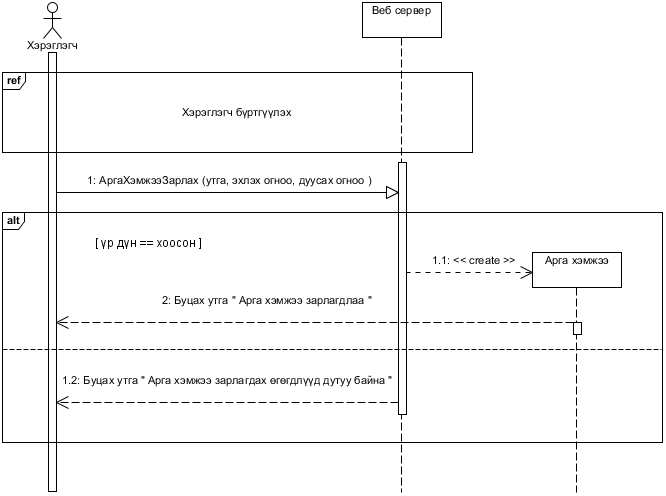
\includegraphics[scale=0.7]{Diagrams/arga_hemjee}
	\caption[Арга хэмжээ зарлах шинжилгээний дарааллын диаграм]{Арга хэмжээ зарлах шинжилгээний дарааллын диаграм}
	\label{text}
\end{figure}

\begin{figure}
	\centering
	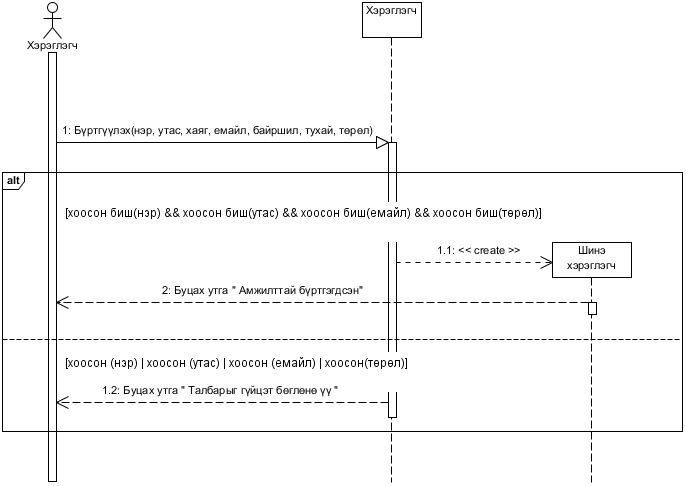
\includegraphics[scale=0.65]{Diagrams/create}
	\caption[Бүртгүүлэх шинжилгээний дарааллын диаграм]{Бүртгүүлэх шинжилгээний дарааллын диаграм}
	\label{text}
\end{figure}

\begin{figure}
	\centering
	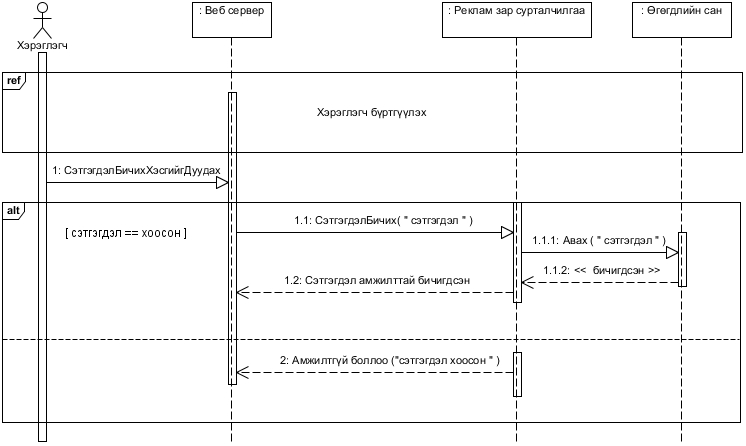
\includegraphics[scale=0.6]{Diagrams/write}
	\caption[Сэтгэгдэл бичих шинжилгээний дарааллын диаграм]{Сэтгэгдэл бичих шинжилгээний дарааллын диаграм}
	\label{text}
\end{figure}

\section{Үйл ажиллагааны диаграм}
\begin{figure}
	\centering
	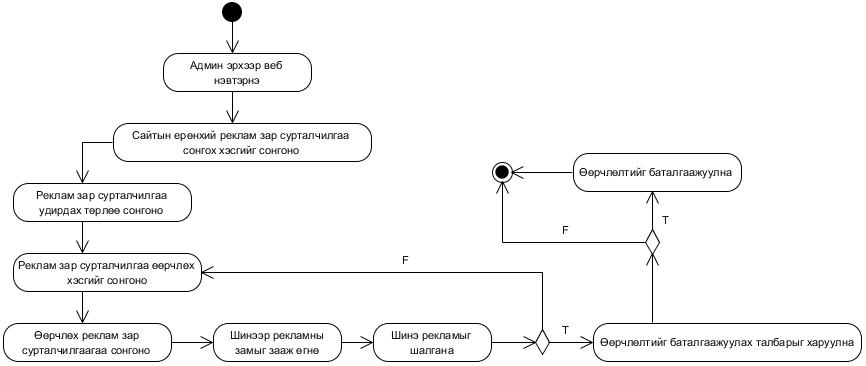
\includegraphics[scale=0.5]{Diagrams/change}
	\caption[Сайтын ерөнхий реклам удирдах үйл ажиллагааны диаграм]{Сайтын ерөнхий реклам удирдах үйл ажиллагааны диаграм}
	\label{text}
\end{figure}
\begin{figure}
	\centering
	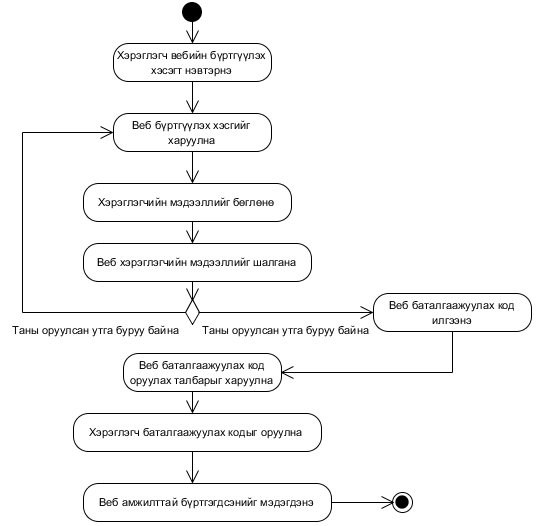
\includegraphics[scale=0.75]{Diagrams/sign_up}
	\caption[Бүртгүүлэх үйл ажиллагааны диаграм]{Бүртгүүлэх үйл ажиллагааны диаграм}
	\label{text}
\end{figure}
\begin{figure}
	\centering
	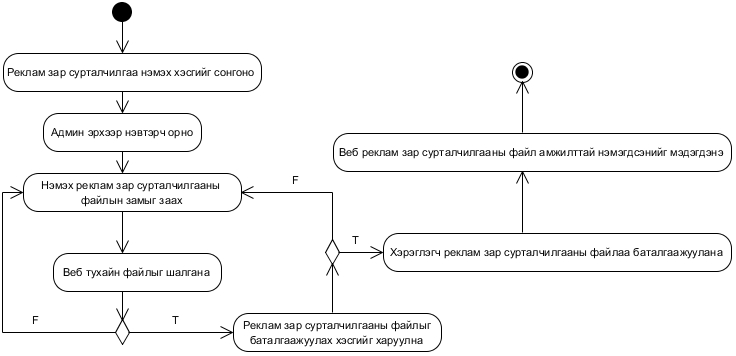
\includegraphics[scale=0.6]{Diagrams/add}
	\caption[Реклам зар сурталчилгаа нэмэх үйл ажиллагааны диаграм]{Реклам зар сурталчилгаа нэмэх үйл ажиллагааны диаграм}
	\label{text}
\end{figure}
\begin{figure}
	\centering
	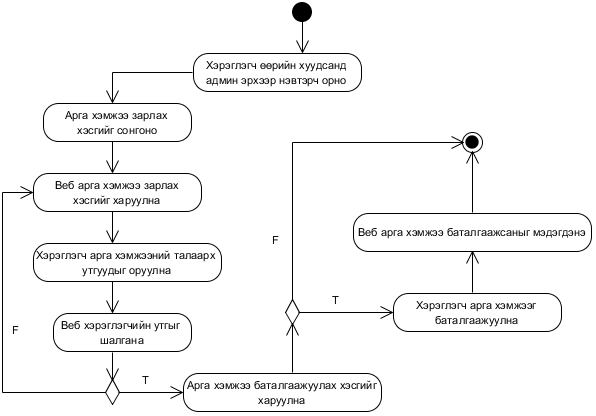
\includegraphics[scale=0.75]{Diagrams/event}
	\caption[Арга хэмжээ зарлах үйл ажиллагааны диаграм]{Арга хэмжээ зарлах үйл ажиллагааны диаграм}
	\label{text}
\end{figure}
\begin{figure}
	\centering
	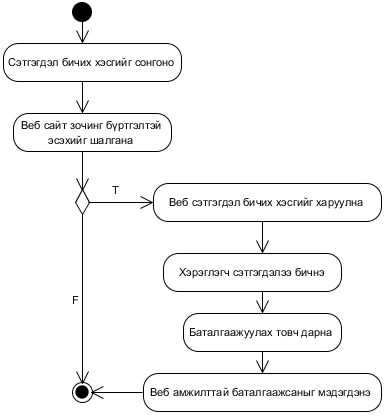
\includegraphics[scale=0.75]{Diagrams/comment}
	\caption[Сэтгэгдэл бичих үйл ажиллагааны диаграм]{Сэтгэгдэл бичих үйл ажиллагааны диаграм}
	\label{text}
\end{figure}w

\begin{figure}
	\centering
	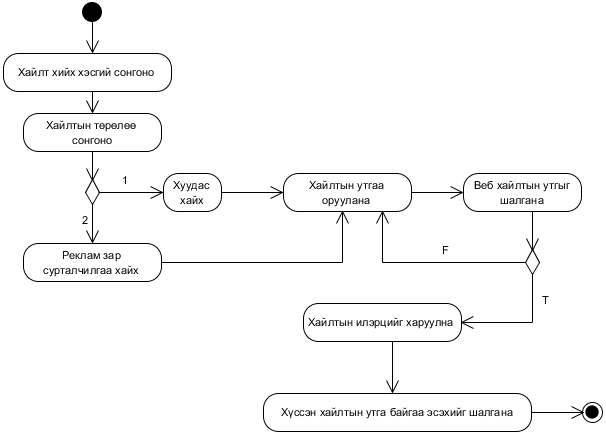
\includegraphics[scale=0.7]{Diagrams/search}
	\caption[Хайлт хийх үйл ажиллагааны диаграм]{Хайлт хийх үйл ажиллагааны диаграм}
	\label{text}
\end{figure}


\section{Бүлгийн дүгнэлт}
Хэрэглэгчийн шаардлагаа тодорхойлж тодорхойлсон шаардлага бүрээ нягтлан хянаж функционал болон фунционал бусаар нь ялгасан. Функционал шаардлага дээрээ үндэслэн юз кейс диаграмаа гаргасан ба бүх  юзкейс бүрт тодорхойлолт гаргасан. Мөн тодорхойлолт бичсэн юзкейс диаграм бүртээ үйл ажиллагааны диаграм зурсан үйл ажиллагааг нь илүү нарийн ойлгомжтой болгож өгч байна.

